%llibreries
\documentclass[12pt,spanish]{article} 
\usepackage[utf8]{inputenc}
\usepackage[OT1]{fontenc}
\usepackage[spanish]{babel}
\usepackage{csquotes}
\usepackage{blindtext}
\usepackage{quotchap}
\usepackage{natbib}
\usepackage{empheq}
\usepackage{babel}
\usepackage{wrapfig}
\usepackage{amsmath}
\usepackage{booktabs} 
\usepackage{lscape}
\usepackage{longtable}
\usepackage{graphicx}
\usepackage{multirow}
\usepackage{circuitikz}
\usepackage{enumerate}
\usepackage[makeroom]{cancel}
\newcommand\tab[1][1cm]{\hspace*{#1}}
\newcommand\unit[1][4pt]{\hspace*{#1}}
\usepackage{float}
\usepackage{listings}
\usepackage{verbatim}
\usepackage{pdfpages}
\usepackage[hidelinks]{hyperref}
\usepackage[margin=2cm]{geometry}
\usepackage{subcaption}
\usepackage{caption}
\usepackage{hyperref}

% Page settings
\usepackage[a4paper,left=20mm, right=20mm,top=20mm,bottom=20mm]{geometry}

\begin{document}

\begin{titlepage}
  \begin{center}
	\includegraphics[scale=0.9]{figures/logoETSIT.png}
	\hfill
	\includegraphics[scale=0.2]{figures/logoGTDM.png}
	\hfill
	\includegraphics[scale=0.3]{figures/logoUPV.png}
	\hfill
    
    \vspace{0.5cm}
    
    \textbf{Grado en Tecnología Digital\\y Multimedia}
    
    \vspace{4cm}
    
    \textbf{Trabajo de final de grado}
    
    \vspace{1cm}
        
    \large
    \textbf{\Huge Diario de desarrollo}
    
    \vspace{0.5cm}
    
    
\includegraphics[scale=0.25]{figures/logo_ai.png}
    
    % subtitle
    
    \vspace{7.5cm}
    
    \textbf{Andreu Llàcer Cantero}


    \vfill
    
  \end{center}
\end{titlepage}

\newpage

\tableofcontents

\newpage

\section{Introducción}

    Al habernos introducido a lo largo del transcurso de la carrera a la tecnología de Motion Capture, se propuso, junto a un compañero, realizar un videojuego que implementara las animaciones 3D realizadas con la tencología anteriormente mencionada.

    En este documento se tratará el trabajo de programación e implementación de todo tipo de material a través de Unity, ya que es el motor gráfico que se ha dado durante la carrera.

\section{Personaje principal}

    El protagonista del videojuego es Andoro, un ingeniero que investiga junto a su compañero Salinas el viaje interdimensional, abriendo la puerta al multiverso.

    Durante el transcurso del videojuego, adquirirá varias habilidades que le ayudarán a defenderse por los distintos universos.\\

    Para implementar el control del jugador se empleará el New Input System de Unity, para poder adaptarlo tanto para mando como para teclado.

    El esquema de controles implementado es el siguiente:

\begin{table}[!h]
\centering
\begin{tabular}{c|c|c|}
\cline{2-3}
                                                 & Teclado y ratón       & Mando              \\ \hline
\multicolumn{1}{|c|}{Movimiento}                 & Teclas WASD           & Joystick izquierdo                   \\ \hline
\multicolumn{1}{|c|}{Mirar}                      & Posición del ratón    & Joystick derecho                     \\ \hline
\multicolumn{1}{|c|}{Salto}                      & Tecla espacio         & Botón inferior                       \\ \hline
\multicolumn{1}{|c|}{Sprint}                     & Tecla shift izquierda & Botón derecho                        \\ \hline
\multicolumn{1}{|c|}{Ataque rápido}              & Click derecho         & Botón izquierdo                      \\ \hline
\multicolumn{1}{|c|}{Ataque lento}               & Tecla Q               & Botón superior                       \\ \hline
\multicolumn{1}{|c|}{Ataque a distancia}         & Click izquierdo       & Gatillo derecho                      \\ \hline
\multicolumn{1}{|c|}{Cambio de arma}             & Tecla Tabulador        & Teclas horizontales de la cruceta    \\ \hline
\multicolumn{1}{|c|}{Interactuar con el entorno} & Tecla E               & Botón superior                       \\ \hline
\end{tabular}
\caption{Controles del personaje}
\end{table}

\newpage

\subsection{Control de personaje}

\subsubsection{Movimiento}

\subsubsection{Mirar}

\subsubsection{Salto}

\subsubsection{Sprint}

\newpage

\subsection{Combate}

    Para el combate se han implementado tres tipos de armas con sus respectivas habilidades y estadísticas para contar con diferentes estilos de combate. Estas tres armas son:

    \textbf{Espada:} Con esta arma el objetivo es que el combate sea un poco más lento, pero a cambio se inflingirá un mayor daño.

    \textbf{Escudos:} Este es el estilo de combate más rápido y ágil, aunque con menos daño.

    \textbf{Bastón:} Estilo de ataques a distancia, pensado principalmente para los enemigos aéreos o para inflingir daño en área cuando haya agrupaciones de enemigos.

\subsubsection{Cambio de arma}

    La función de cambio de arma opera a través de una máquina de estados que alterna entre las tres armas según si indicamos cambiar a la siguiente arma o a la anterior, siempre en el mismo orden.

    Los ataques que el jugador utiliza durante el juego, revisan en primera insatancia el arma que se esté usando en el momento del ataque, para así realizar la animación correcta con el daño correspondiente.

\subsubsection{Ataque rápido}

    El ataque rápido, en los tres estilos, es un golpe cuerpo a cuerpo con una animación breve para poder usarse de forma recurente y sin que tome demasiado tiempo.

    En el caso del escudo y la espada, presionar el botón de ataque rápidamente hará que combinemos distintos golpes hasta el tercer pulsamiento, completando un combo.

    En el caso del bastón, al no estar pensado para usar principalmente en combate cercano, simplemente alterna la dirección del bastonazo.\\

    Para implementar esta mecánica, se activa un temporizador al presionar el ataque por primera vez. Si este temporizador no ha bajado a cero cuando volvamos a pulsar el botón de ataque, se activará la animación del segundo golpe del combo. El tercer golpe funcionará de la misma forma, siendo este el que causa un daño mayos y reiniciando el contador de golpes para que al volver a pulsar el botón de ataque, la animación sea la del primer ataque.

\subsubsection{Ataque lento}

    Con este ataque se busca que el jugador tenga que decidir bien el momento en el que lo utilice, ya que al realizarse, este cancelará el movimiento durante su ejecución, dejándolo brevemente expuesto a ataques enemigos.\\

    Existe la posibilidad de combinar este ataque con la sucesión de ataques rápidos para activar un ataque de combo distinto al que aparece al combinar tres pulsaciones de ataque rápido.

\newpage

\subsubsection{Ataque a distancia}

    El ataque a distancia consiste en un breve proyectil en caso de estar usando la espada o los escudos, con una animación corta, ya que estos estilos están pensados para el combate cuerpo a cuerpo, y este ataque serviría para aturdir brevemente a los enemigos impiactados y acercarse hasta pque entrasen en rango de nuestro ataques mas potentes. En el caso del bastón, al ser el ataque más potente, tomará una cantidad de tiempo mayor, pero causará un mayor daño.\\

    El proyectil creado según el estilo de combate se instanciará siempre en la dirección en la que estemos mirando. En el caso de estar jugando con el mando, podremos apuntar mientras nos movemos con el joystick derecho, de igual forma que si disparamos con teclado y ratón el personaje se girará para apuntar en la dirección en la que se encuentre el cursor.

\newpage

\subsection{Interacción con el entorno}

\subsubsection{Diálogos}

\subsubsection{Recoger}

\subsubsection{Obervar}

% \begin{figure}[h]
% \begin{subfigure}{.5\textwidth}
%     \centering
%     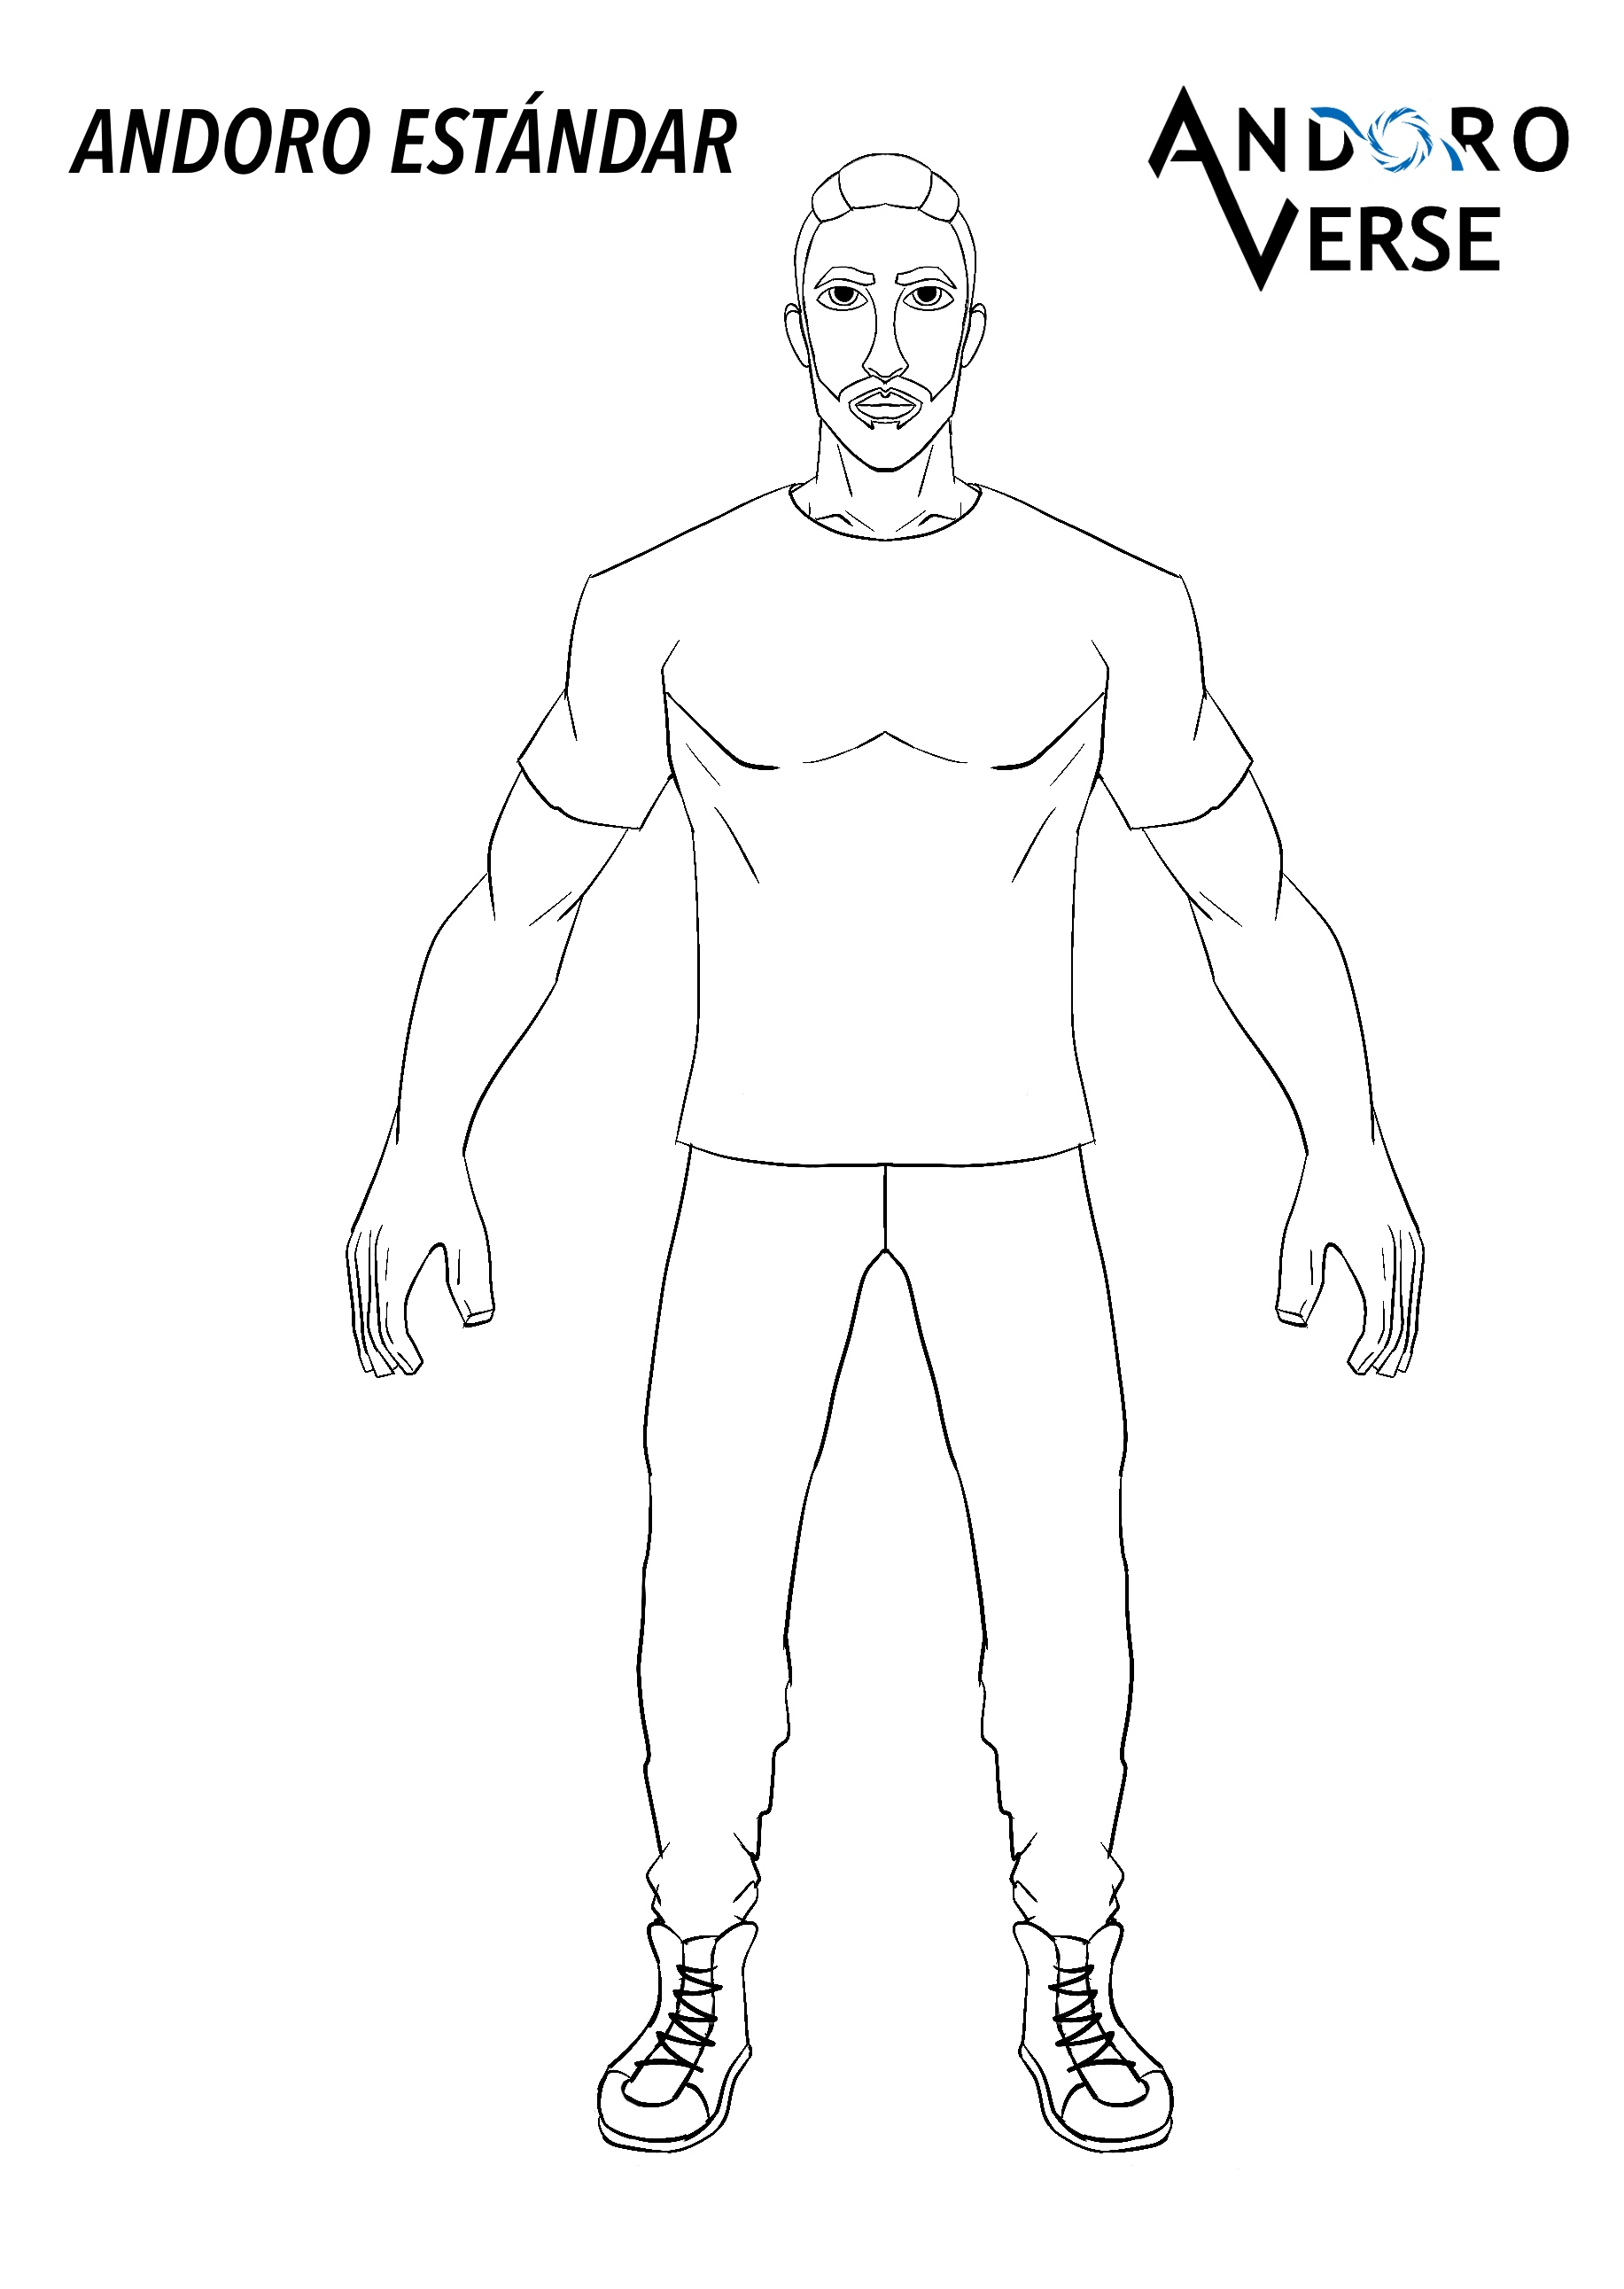
\includegraphics[width=0.75\linewidth]{concepts/doroBase/Andoro_Base.jpg}
%     \caption{Boceto a tinta}
%     \label{fig:corte1}
% \end{subfigure}
% \begin{subfigure}{.5\textwidth}
%     \centering
%     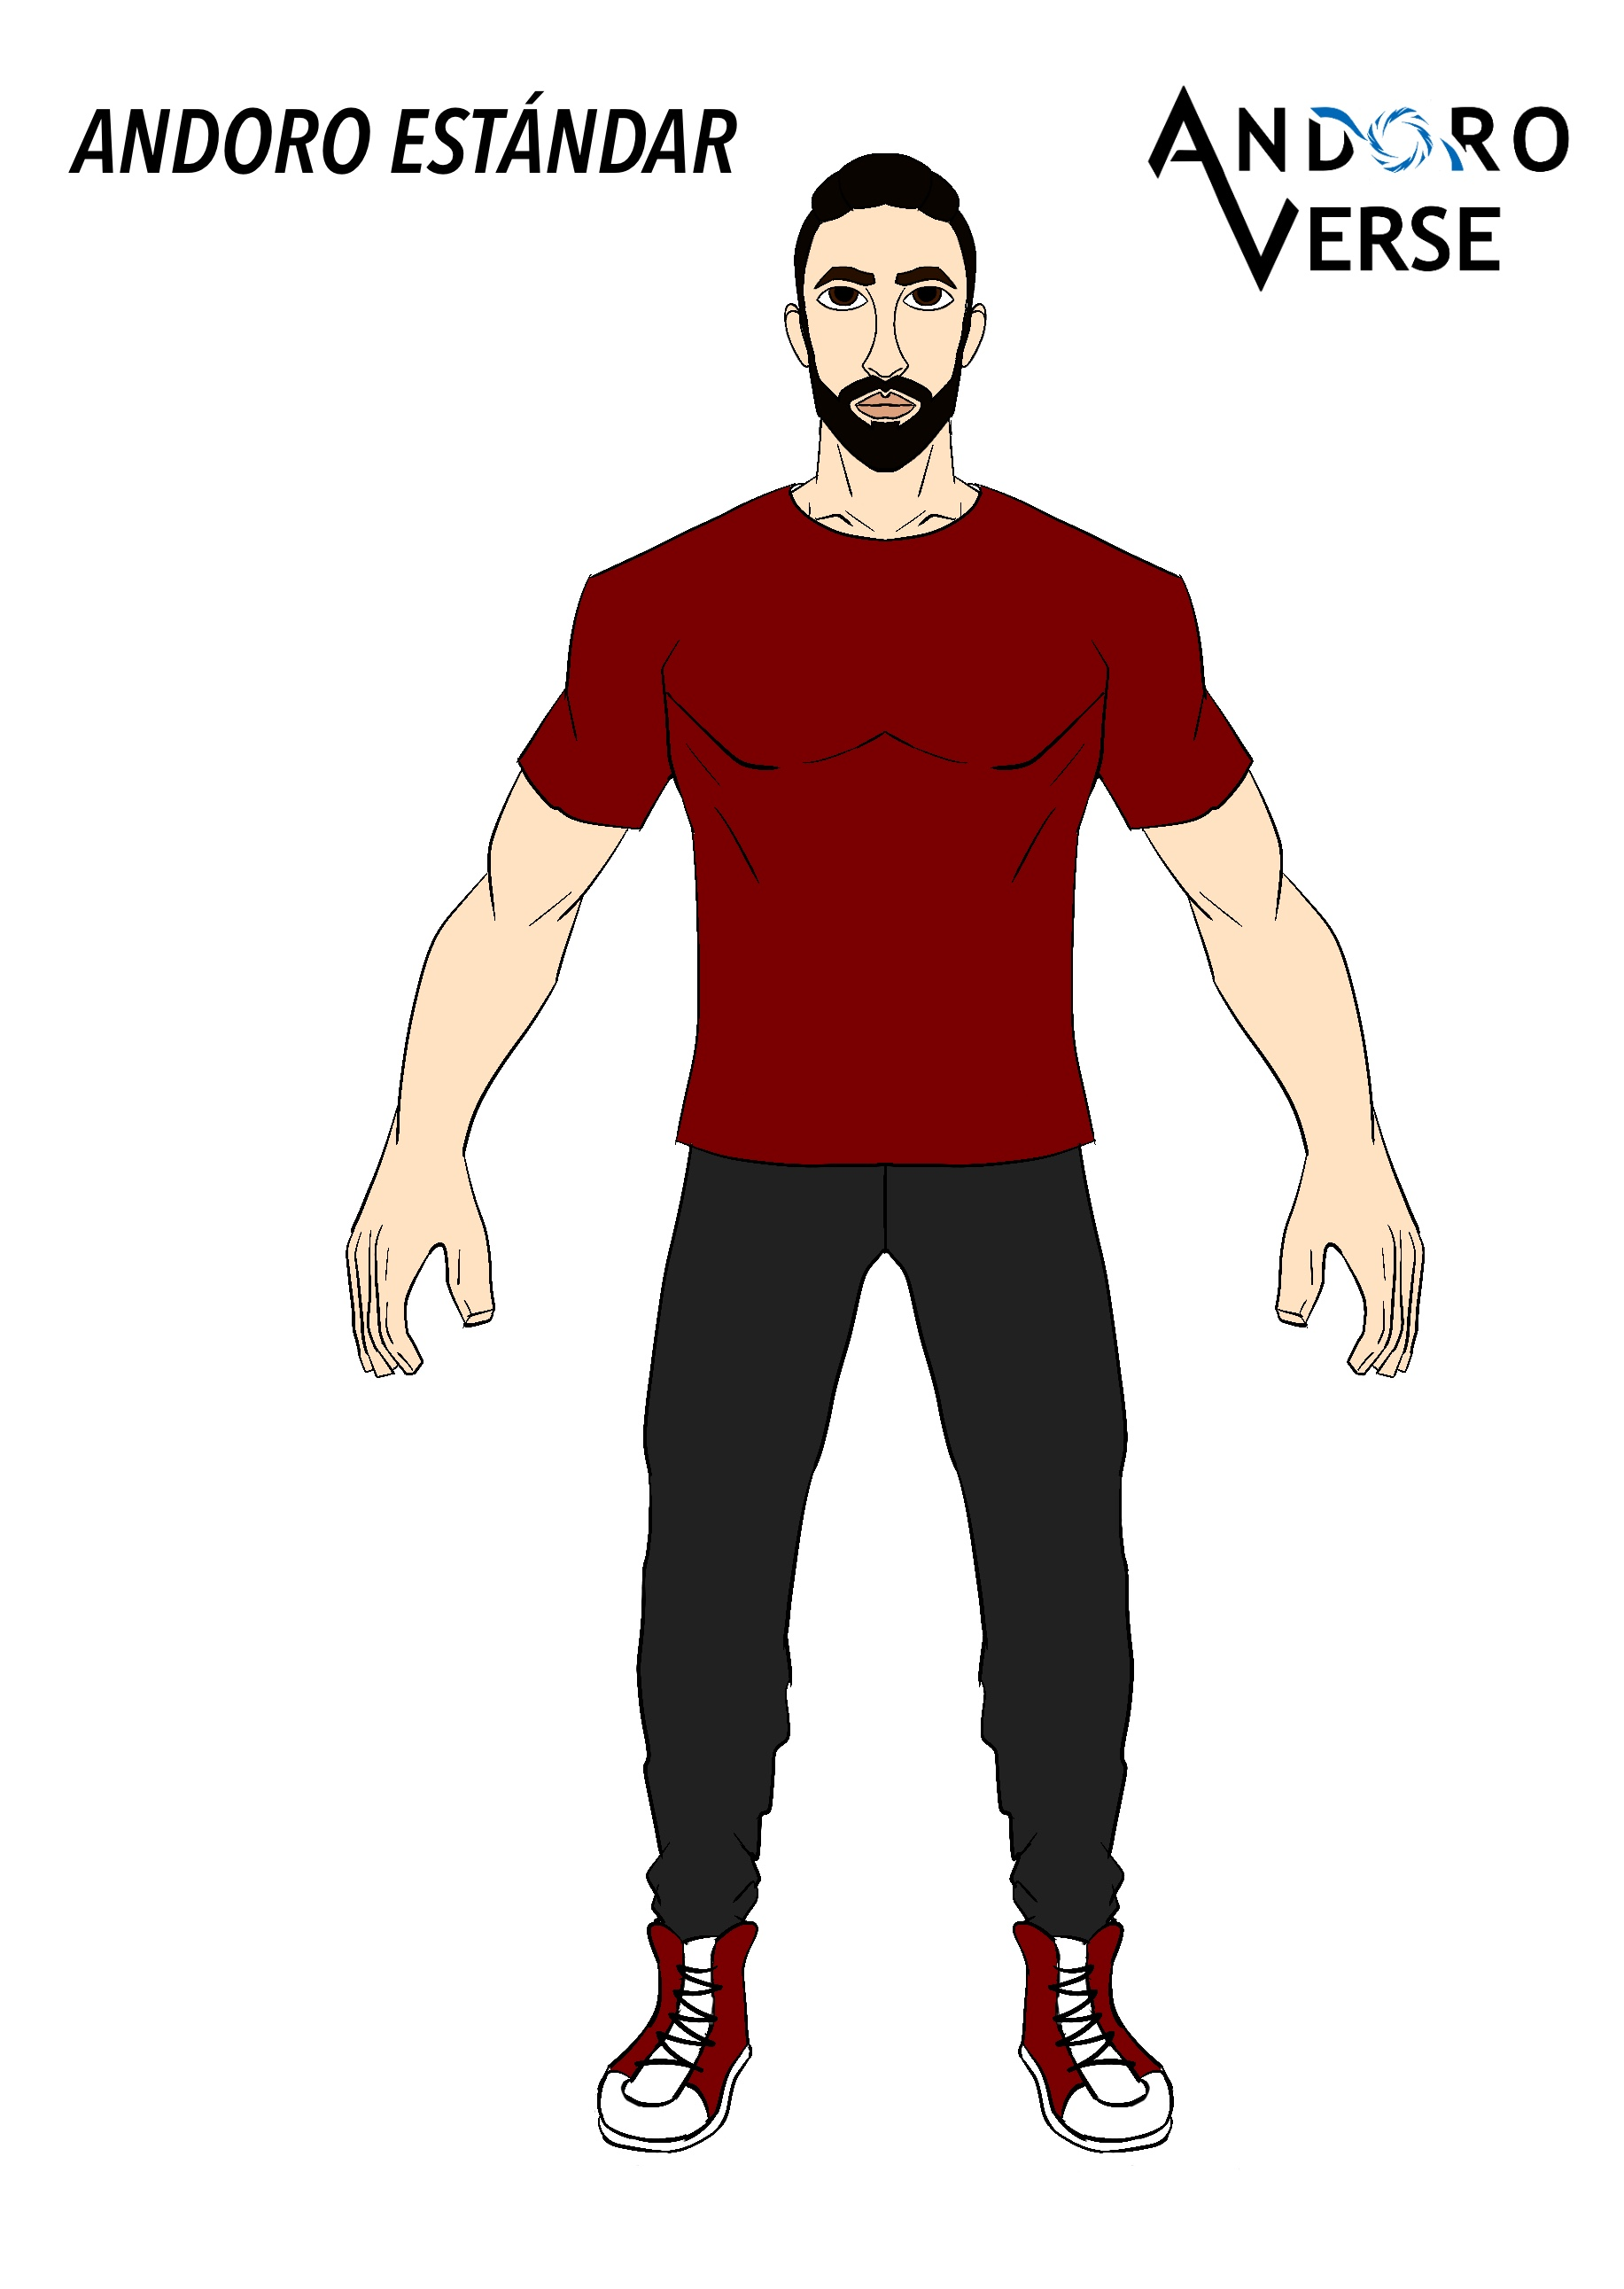
\includegraphics[width=0.75\linewidth]{concepts/doroBase/Andoro_Base (1).jpg}
%     \caption{Boceto a color}
%     \label{fig:corte2}
% \end{subfigure}
% \caption{Primer boceto de Andoro Base}
% \end{figure}
    
%\begin{figure}[h!]
%  \centering
%  \includegraphics[width=0.15\linewidth]{concepts/examples/anderuSketch.jpeg}
%  \caption{Primer boceto de Andreu con el estilo de arte}
%  \label{fig:t2}
%\end{figure}

\newpage

\section{Enemigos}

    Para esta demo del videojuego, se decidió diseñar e implementar un total de tres enemigos:\\

    - AndroSphere

    - CannonFly

    - Mortero\\

    A continuación se resumirán las técnicas y procedimientos empleados para conseguir el correcto funcionamiento de estos elementos del juego.

\subsection{Función de patrullaje}

    Para que el enemigo pueda alternar entre patrullaje, persecución al enemigo o simplemente estar quieto, en todos los scripts que manejan el movimiento de los enemigos se crea una lista con estos tres estados. Más tarde, el código comprueba que en la lista pública dedicada a incluir puntos de patrullaje este o no vacía. En caso de detectar que hay un sitio, simplemente se moverá a esta localización, sin embargo, de haber más posiciones incluidas en la lista, el enemigo entrara en estado "Patrol", alternando la posición en el orden en el que se hayan asignado las posiciones.

\newpage

\subsection{AndroSphere}

\subsubsection{Diseño}

    El primer enemigo se diseñó pensando en un enemigo simple que se acercara a cierta distancia y realizara un ataque cuerpo a cuerpo cada cierto tiempo, así como causar daño al impactar contra el jugador.

\subsubsection{Movimiento}

    Para el movimiento de este enemigo se investigó la forma de que encontrara  de forma automática una ruta hasta la posición del jugador. Para ello, se encontró un paquete experimental llamado "AI Navigation", que proporciona la capacidad de trabajar con varios componentes de Unity que se explicarán a continuación.

\begin{figure}[h!]
 \centering
 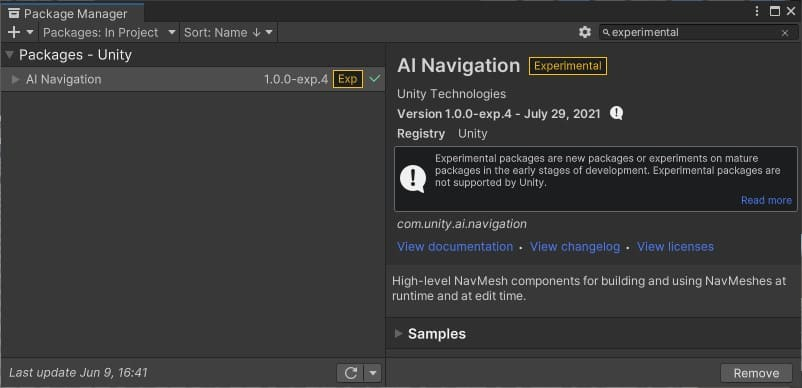
\includegraphics[width = 0.6\linewidth]{enemies/AndroSphere/AINavigation.jpg}
 \caption{Ventana de Package Manager con el paquete experimental AI Navigation}
 \label{fig:t2}
\end{figure}

    La primera parte de este paquete ha consistido en definir un NavMeshAgent cuyos parámetros se adapten al enemigo en cuestión, indicando la altura, radio, inclinación máxima y escalón máximo que puede subir sin tener que lo considere un obstáculo y tenga que buscar una ruta alternativa.

\begin{figure}[h!]
 \centering
 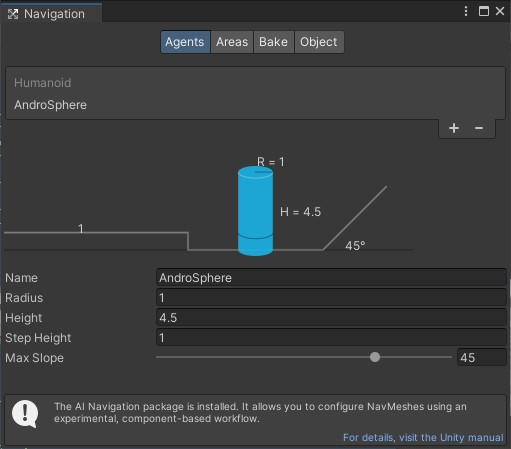
\includegraphics[width = 0.45\linewidth]{enemies/AndroSphere/AndroSphere_NavigationAgent.jpg}
 \caption{Ventana de dfinición del Agente}
 \label{fig:t2}
\end{figure}

\newpage
    
    Con tal de diseñar el movimiento del enemigo, se definió el terreno de prueba cono un NavMeshSurface, haciendo un bake de la superficie seleccionada e indicando los parámetros mínimos que tendrá uno de sus NavMeshAgents para que pueda determinar que zonas de la superficie tienen una inclinación superior a la mínima recorrible por un NavMeshAgent.

\begin{figure}[h!]
 \centering
 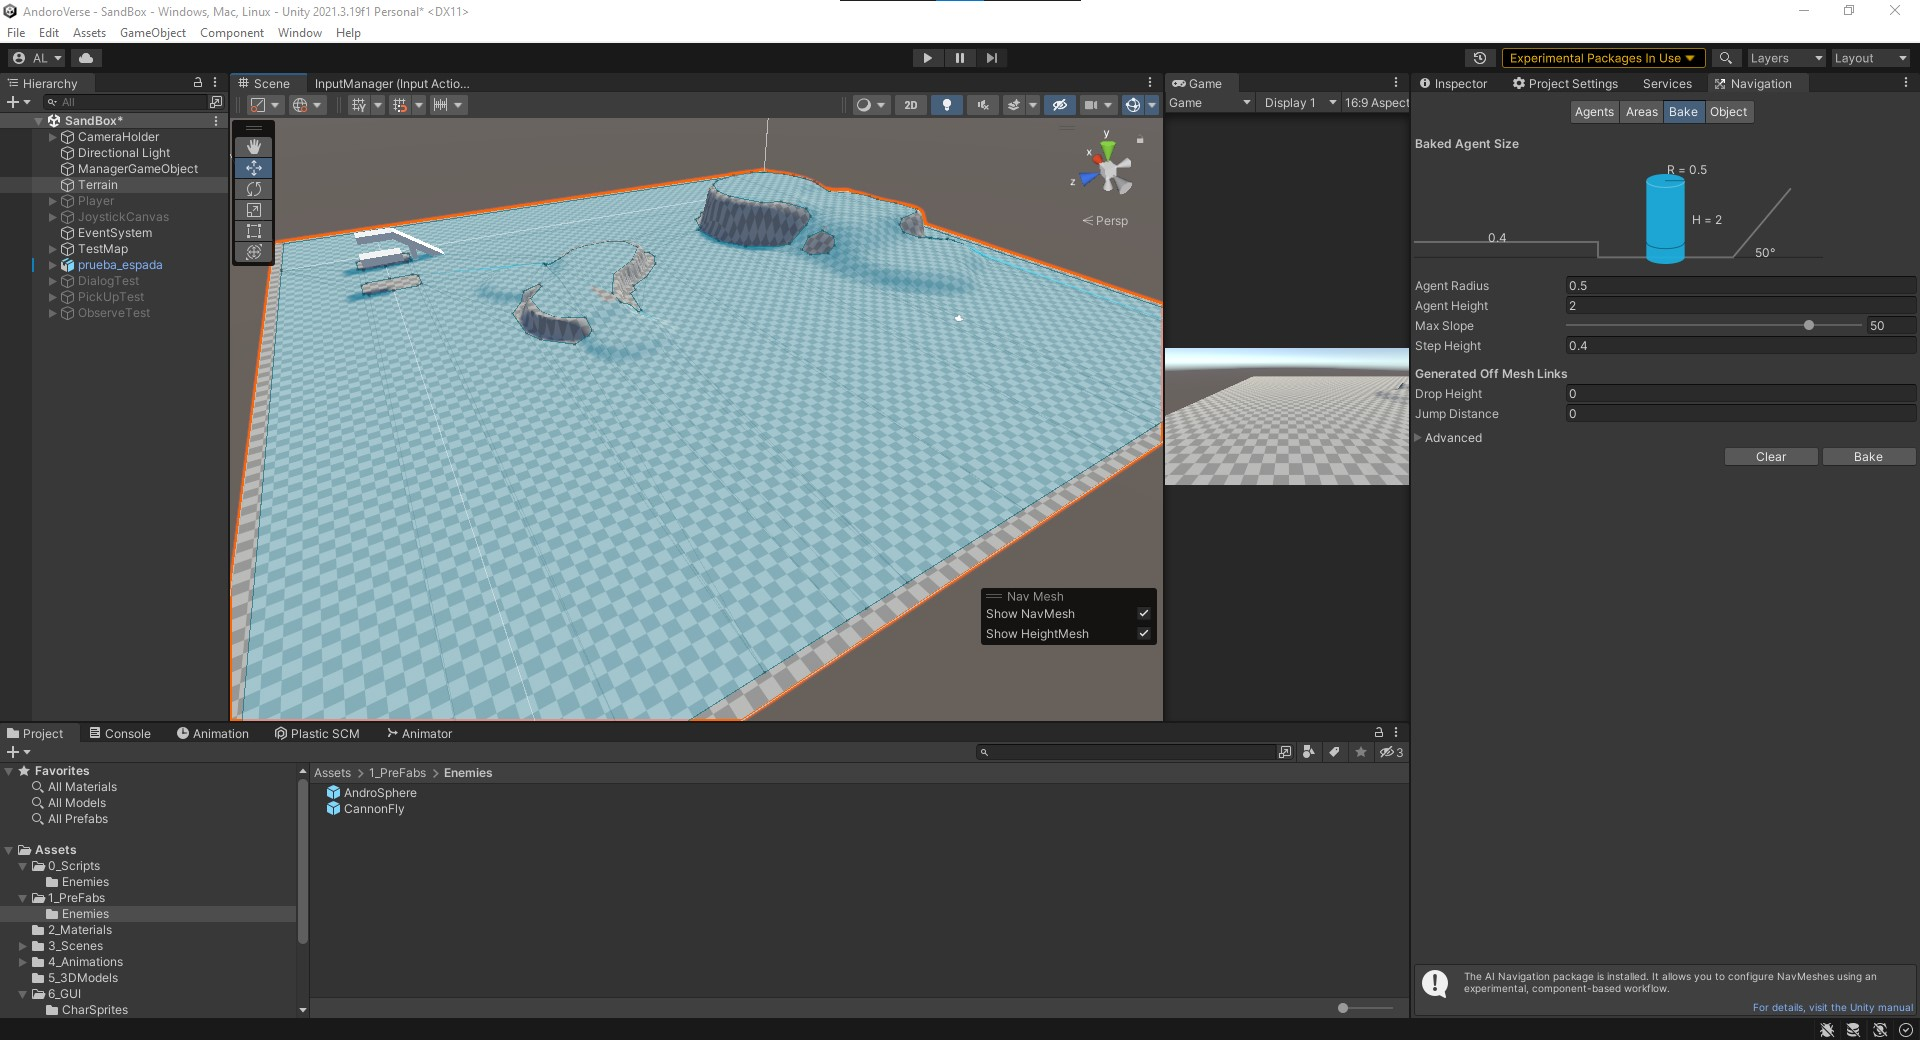
\includegraphics[width = 0.75\linewidth]{enemies/AndroSphere/NavigationWindow.jpg}
 \caption{Terreno de prueba definido como NavMeshSurface}
 \label{fig:t2}
\end{figure}

    Una vez definido el NavMeshAgent del personaje y la superficie sobre la que buscara rutas, solo queda añadir el componente NavMeshAgent y asignar los valores que buscamos, asignando el Agent Type correspondiente.

    El valor en el que queremos fijarnos es el Stopping Distance, ya que este valor nos resulta útil para la función de ataque.

\begin{figure}[h!]
 \centering
 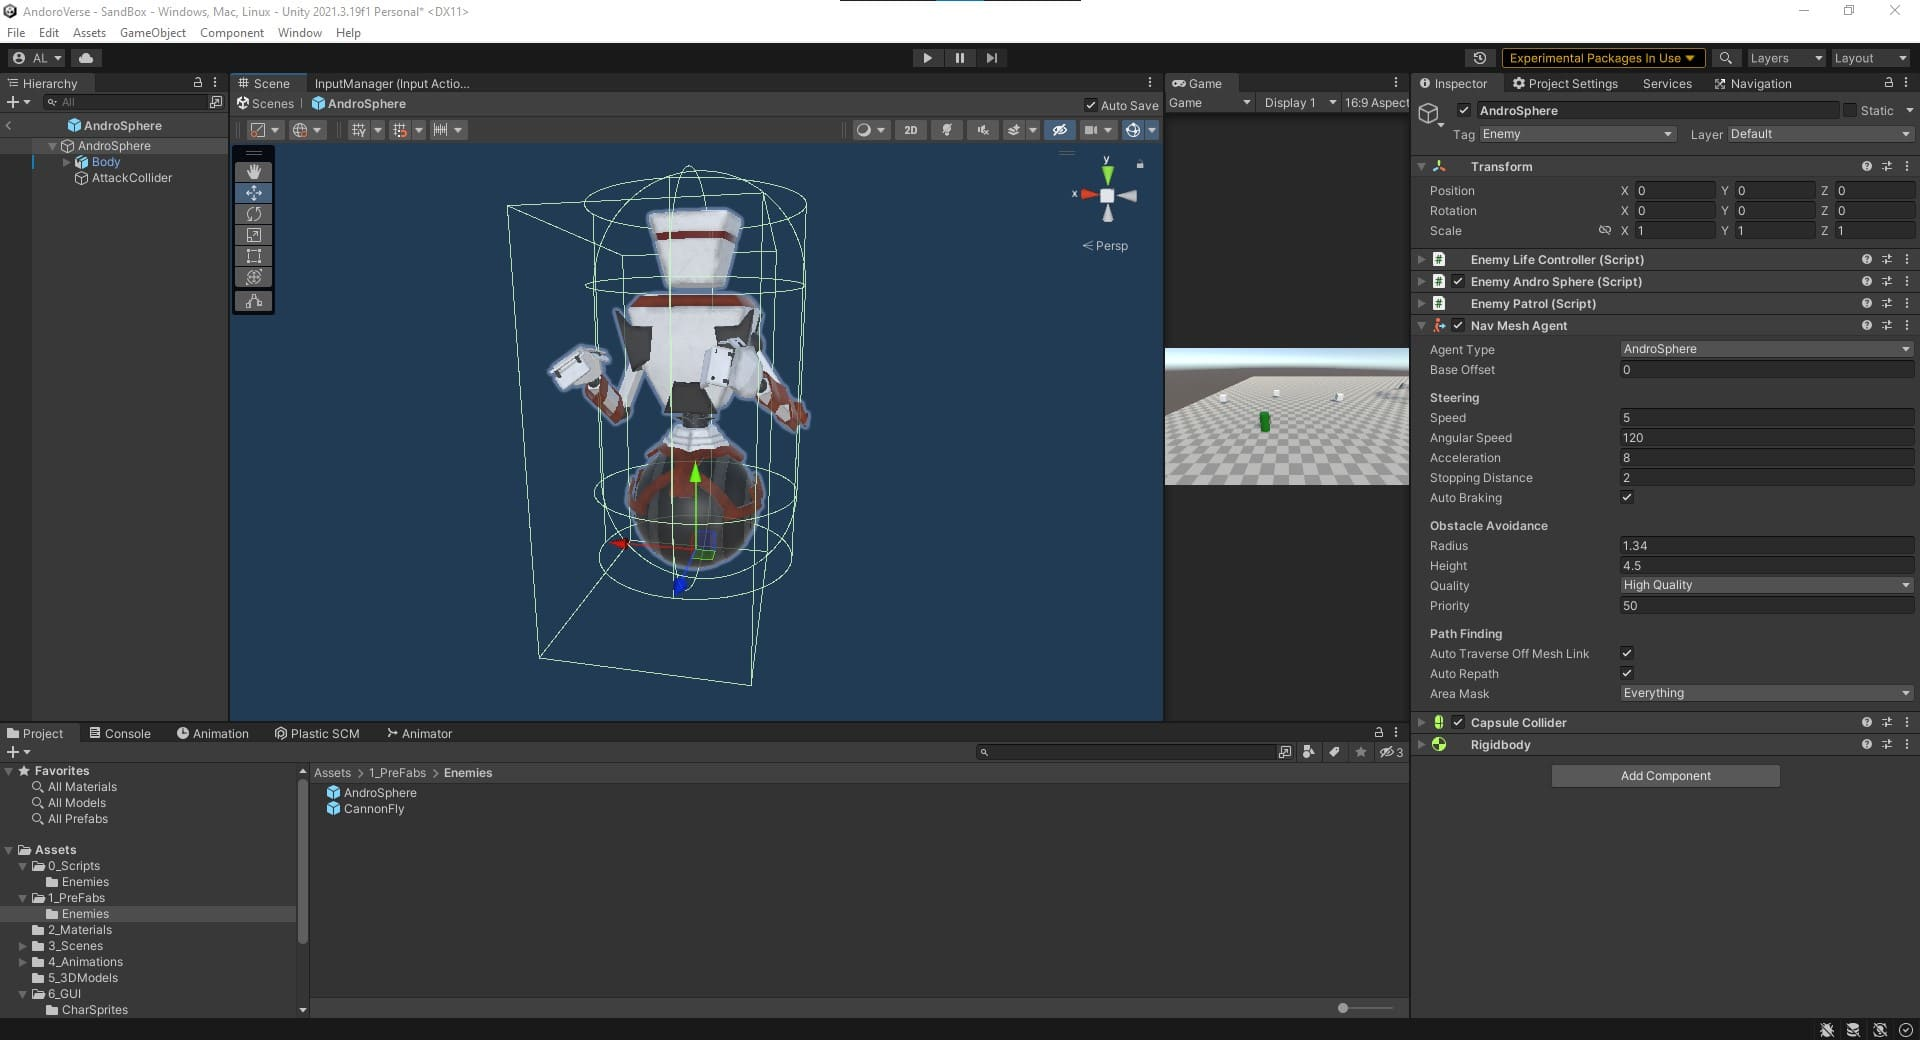
\includegraphics[width = 0.75\linewidth]{enemies/AndroSphere/AndroSphere_NavMeshAgent.jpg}
 \caption{Componente NavMeshAgent}
 \label{fig:t2}
\end{figure}


    Tras aplicar estos pasos con las características que buscamos, solamente debemos indicar en el Script que controle el personaje cuando debe asignar como objetivo la posición del jugador y buscar la ruta más corta hasta este.
    
\newpage

\subsubsection{Ataque}

    Al completar el acercamiento al jugador a una distancia igual o menor a la indicada en el componente NavMeshAgent, se ejecutará la función de ataque. Una corrutina en la que se reproduce la animación de golpeo del AndroSphere y se activa el collider incluido para ser la zona en la que el jugador recibirá una cierta cantidad de daño.

    Cuando el enemigo esta realizando la animación de golpeo, no se movera, y tras completar la animación tomará un breve espacio de tiempo para volver a activar el buscador de ruta hasta el jugador.

\newpage

\subsection{CannonFly}

\subsubsection{Diseño}

    Este enemigo se diseñó buscando un enemigo a distancia desde una posición elevada. Para acrecentar el uso de distintas armas, ese enemigo podrá ser atacado de forma más sencilla con el bastón, ya que su ataque a distancia tiene un daño mayor.
    
\subsubsection{Movimiento}

    Este enemigo tiene como característica que trata de mantener la distancia con el jugador. Para ello se definieron varias distancias:\\

% \begin{wrapfigure}{r}{0.2\textwidth}
%   \begin{center}
%  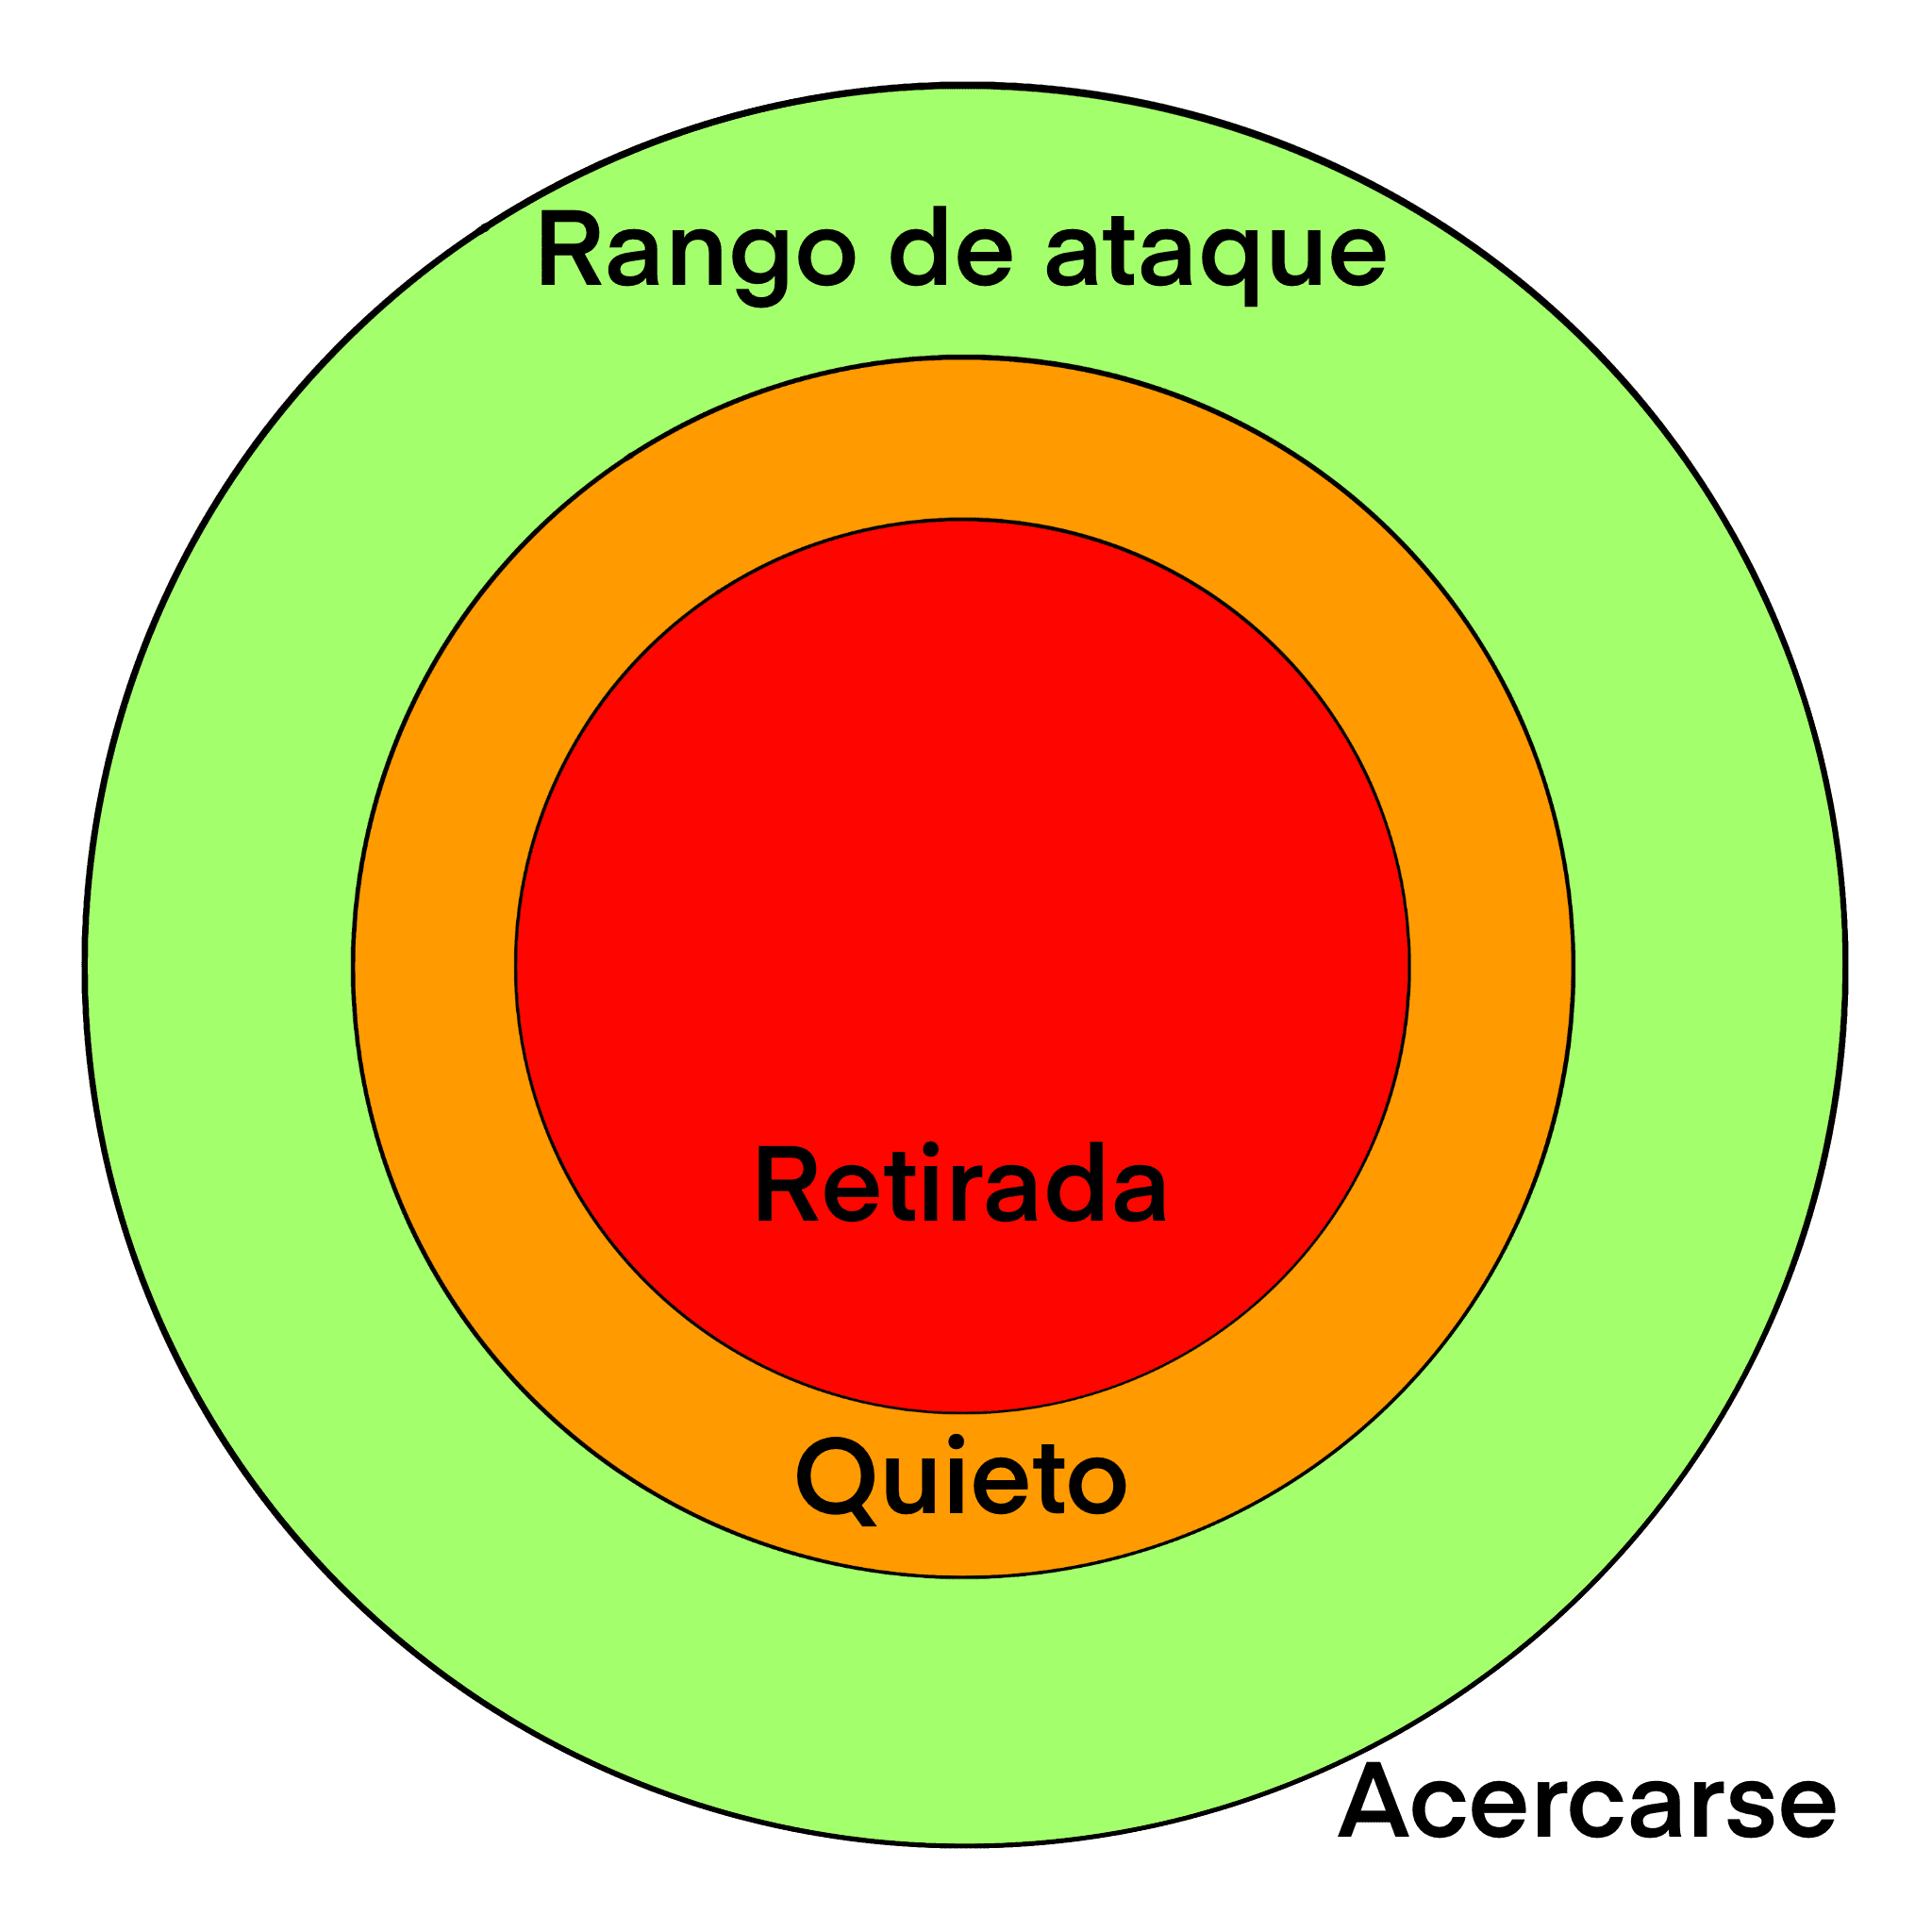
\includegraphics[width = 1\linewidth]{enemies/CannonFly/Rangos.png}
%  \caption{Esquema de las distancias}
%   \end{center}
% \end{wrapfigure}

    - Distancia de rango: Una distancia menor a este valor indicará al enemigo que el jugador esta a rango de ser disparado.

    - Distancia mínima: Distancia mínima a la que el enemigo puede estar del jugador. En el momento en el que la distancia sea menor a este valor, el enemigo tratará de ganar terreno, alejándose del jugador.

    - Distancia máxima: Distancia en la que el enemigo no necesita acercarse más al jugador y puede estar quieto hasta que la distancia sea menor de la permitida. Con estos evitamos que la distancia mínima tenga que ser un único valor y que por tanto tiemble por mantener siempre el mismo valor.

\begin{figure}[h!]
 \centering
 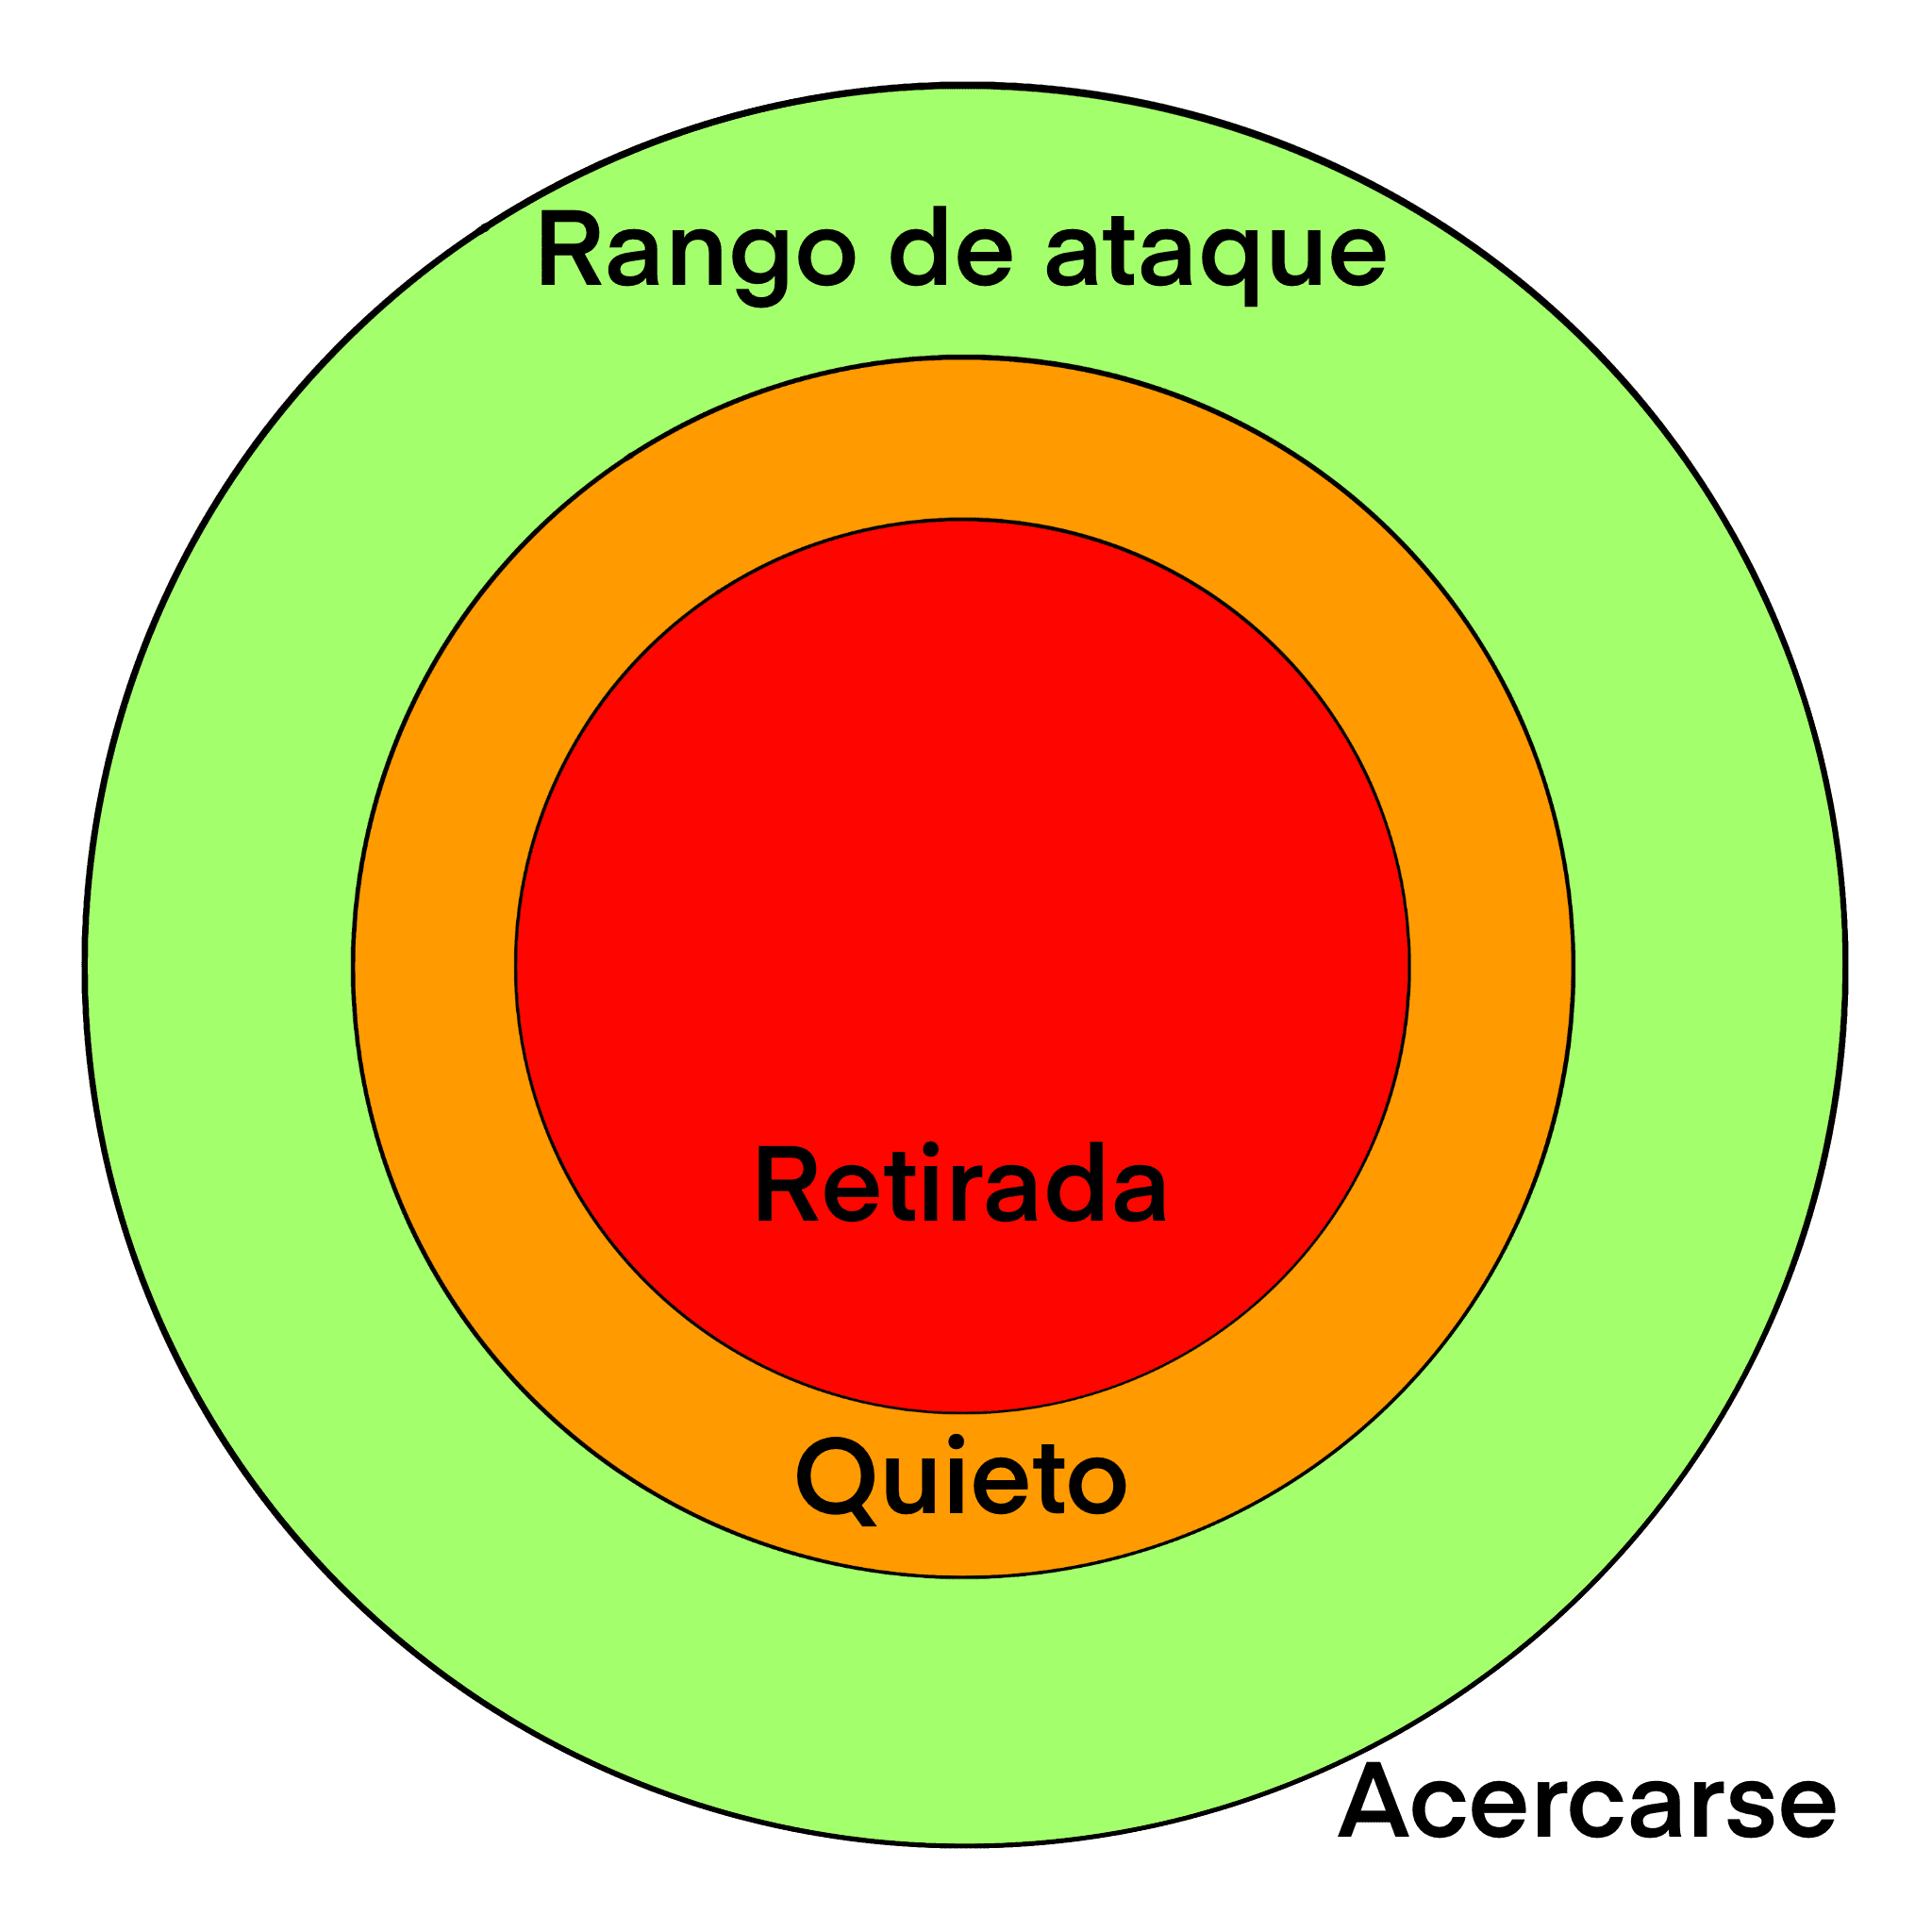
\includegraphics[width = 0.25\linewidth]{enemies/CannonFly/Rangos.png}
 \caption{Esquema de las distancias}
 \label{fig:t2}
\end{figure}

    Con estos valores, el script maneja el enemigo para que mantenga las distancias, pero sin retirarse a una velocidad mayor a la del jugador, ya que en tal caso estaríamos persiguiendo hasta la saciedad al enemigo.\\

\newpage

    Además de mantener la distancia con el jugador en el plano horizontal, se ha añadido una función en la que se lanza un "Raycast" hacia el suelo, detectando así si hay suelo o no. En caso de tener contacto con un elemento que tenga asignada la máscara ``Terrain" asignada, la altura del dron subirá ligeramente. Por el contrario, si el raycast no detecta suelo al final de este, el dron reducirá la altura hasta que el raycast tenga un contacto.

\begin{figure}[h!]
 \centering
 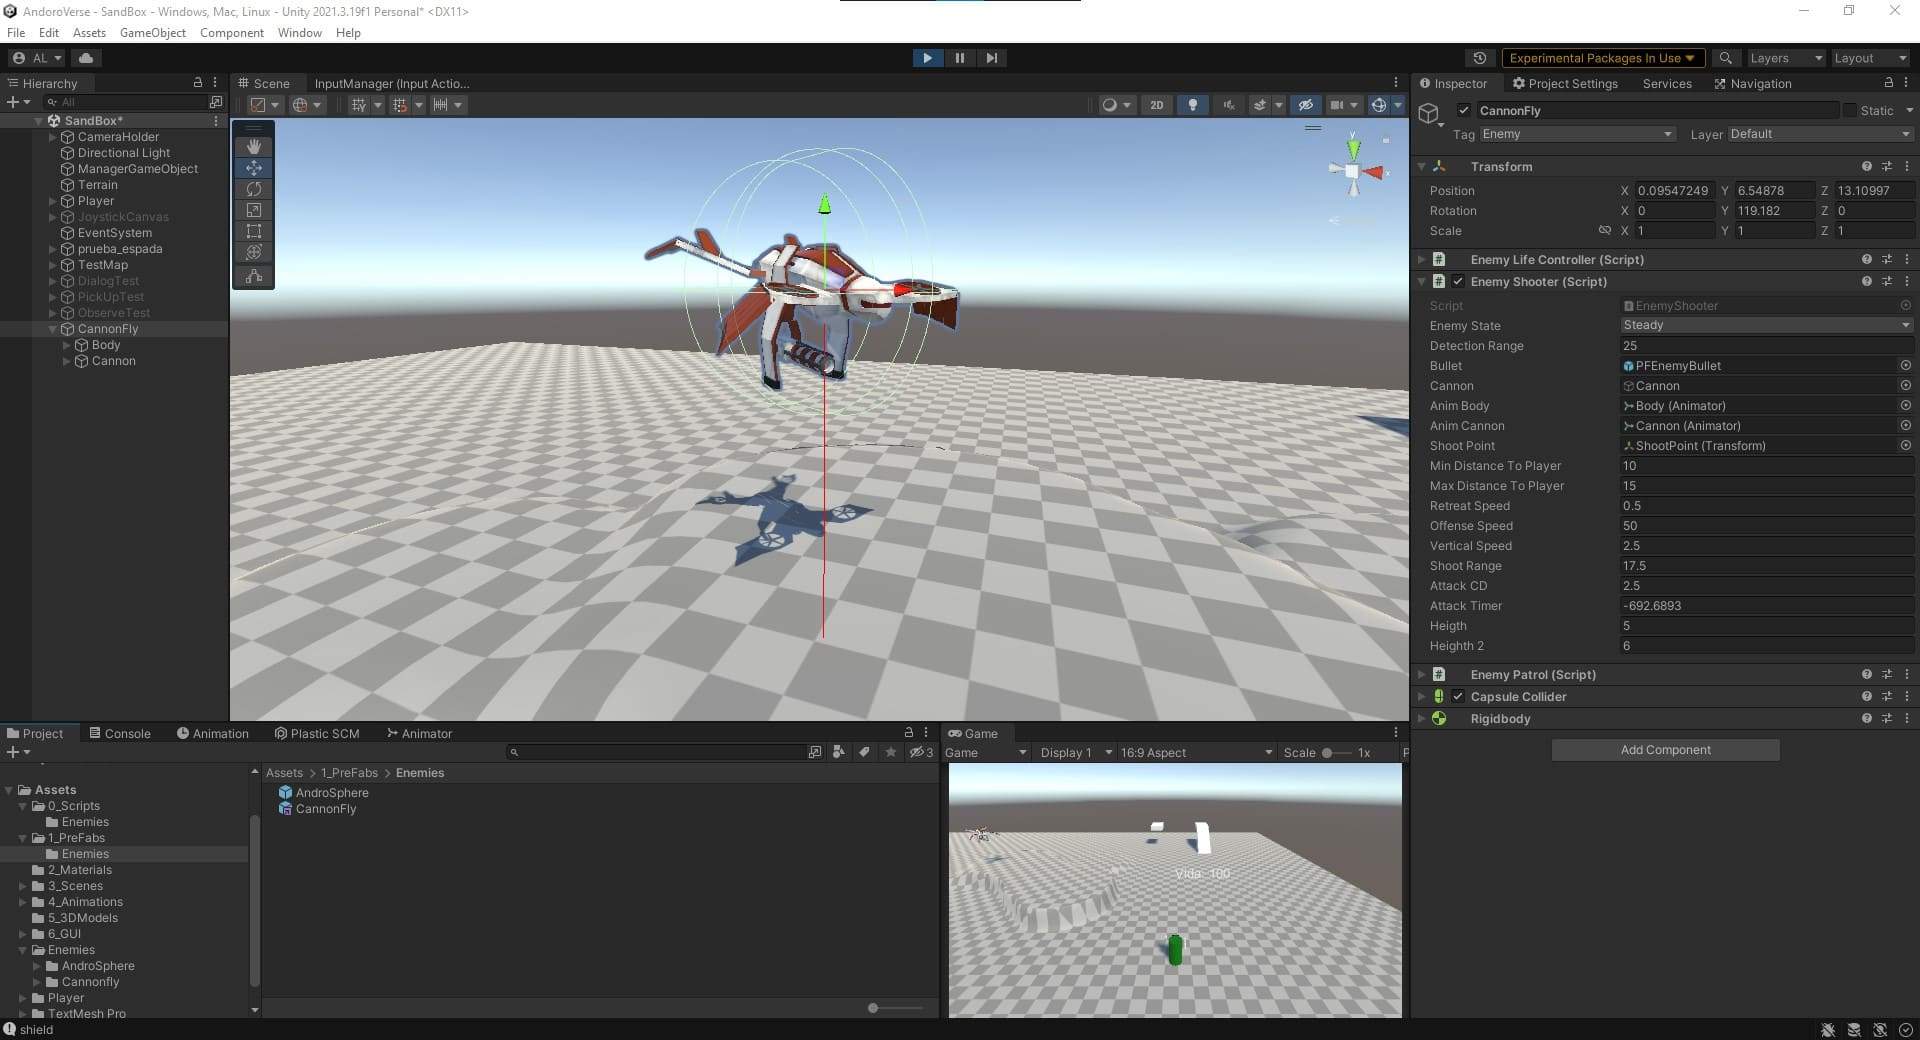
\includegraphics[width = 0.7\linewidth]{enemies/CannonFly/CannonFly_Raycast.jpg}
 \caption{Raycast para medir la altura}
 \label{fig:t2}
\end{figure}

\subsubsection{Ataque}

    Al tratarse de un enemigo con ataques a distancia, la función de ataque es tan simple como crear un PreFab de un GameObject. En este caso, para el proyectil se creo una cápsula junto con un script que hace que se mueva recto, con la orientación que se le proporcione al momento de crearla, hasta que bien impacta contra un objeto que causa su destrucción, como puede ser un muro o el propio personaje, al que causará un cierto daño, o bien pasados unos segundos. También se le añadió un sistema de particulas en la parte trasera.

\begin{figure}[h!]
 \centering
 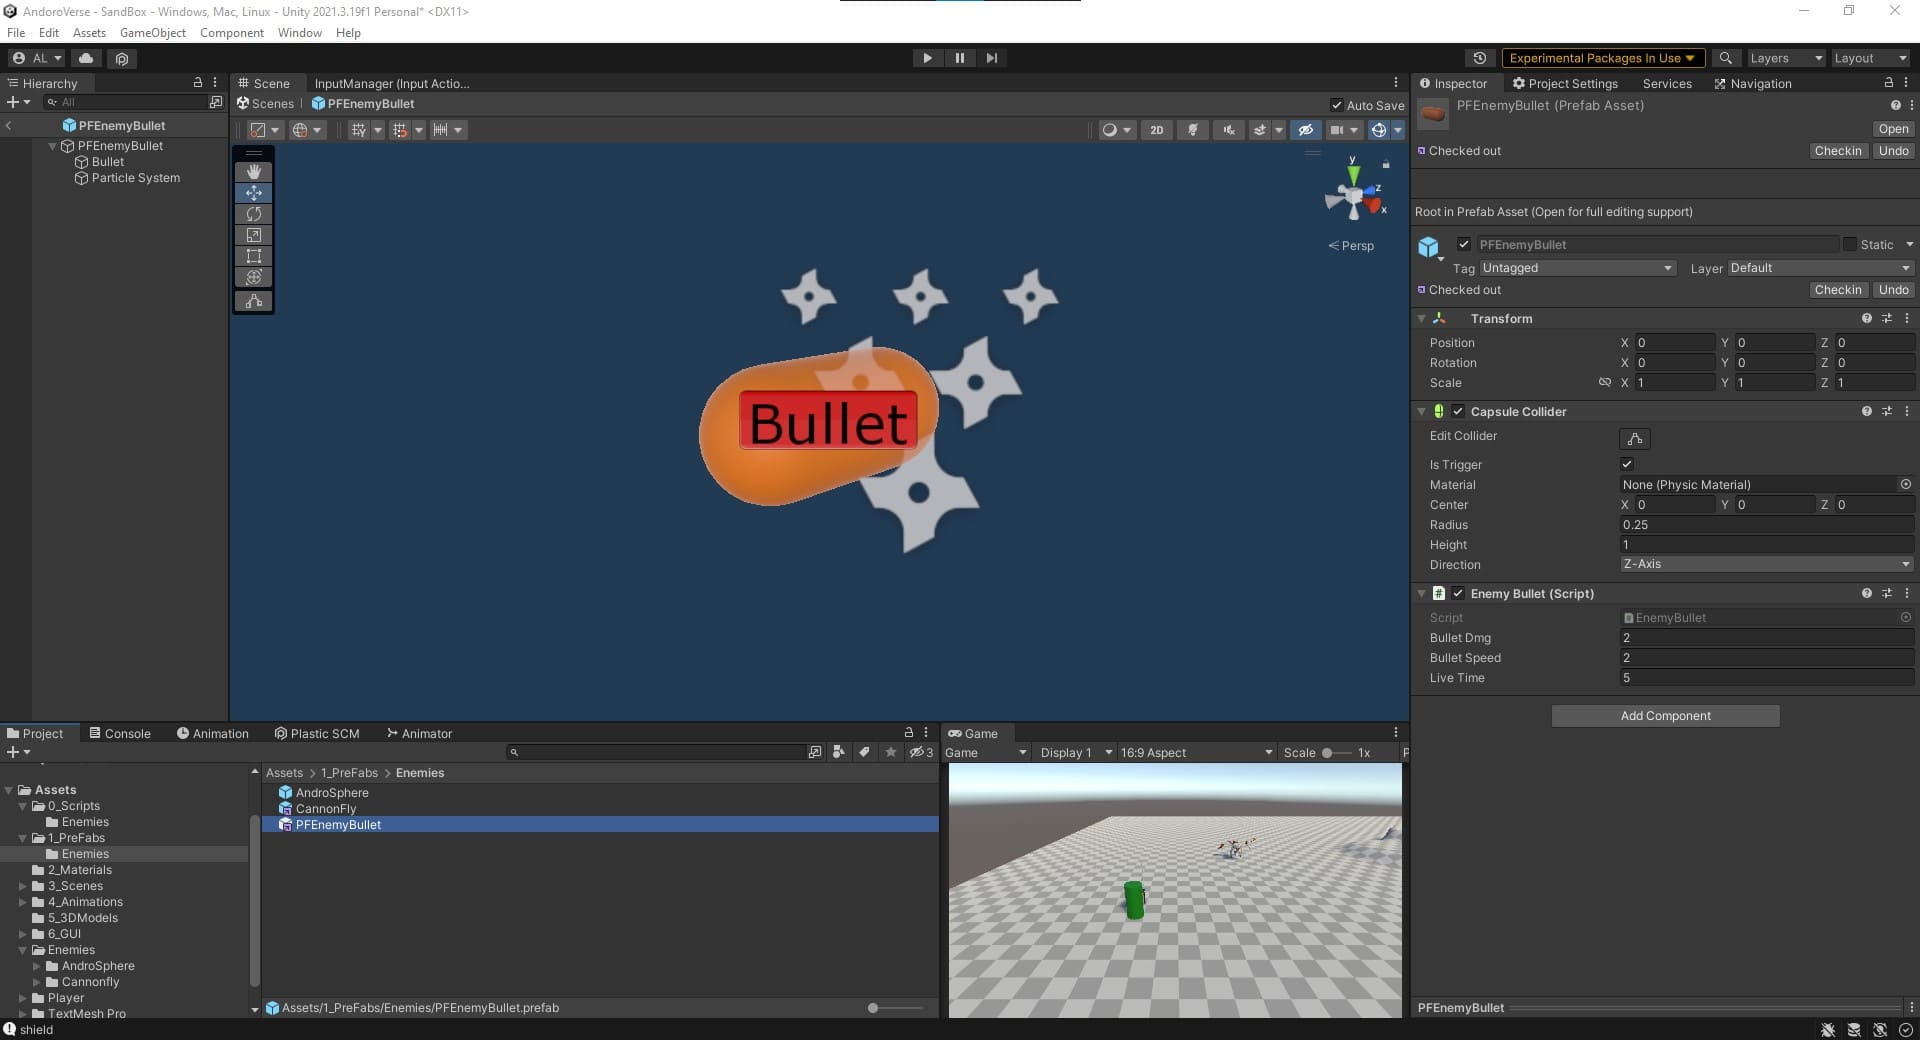
\includegraphics[width = 0.7\linewidth]{enemies/CannonFly/CannonFly_Bullet.jpg}
 \caption{PreFab de la bala}
 \label{fig:t2}
\end{figure}

\newpage

    Para implementar las animaciones del modelo, se dividió a este en dos partes. Una consiste en el cuerpo principal del dron, mientras que la otra viene a ser colamente el cañón. El motivo de este es que se buscaba que el cuerpo rotara para encarar siempre al jugador o al punto al que se esta dirigiendo en caso de patrullaje, mientras que el cañón solamente se moverá en un eje apuntando al jugador cuando este estuviera en rango.

\newpage

\subsection{Mortero}

\subsubsection{Diseño}

\subsubsection{Movimiento}

\subsubsection{Ataque}

\newpage

\section{Interfaz}

\subsection{Menú inicial}

\subsection{Menú de pausa dentro del juego}

\newpage

\section{Entornos y mapa}

\newpage

\section{Webgrafía}

\href{https://www.youtube.com/watch?v=dQw4w9WgXcQ}{[1] Stable-Diffusion explanaition}\\

\end{document}